\section{Vector Equation of Lines}

\begin{definition}[Vector Equation of Lines]
	The {\bf position vector} of $\underline{x}$ of an arbitrary point P(x,y,z) on the line in terms of $\underline{p}$ and $\underline{v}$
	\begin{equation}
		\label{eq: vector-lines}
		\underline{x} = \underline{p} + t\underline{v} \ \ \ \ \text{for } t \in \mathbb{R}
	\end{equation}
\end{definition}

\begin{figure}[H]
	\centering
	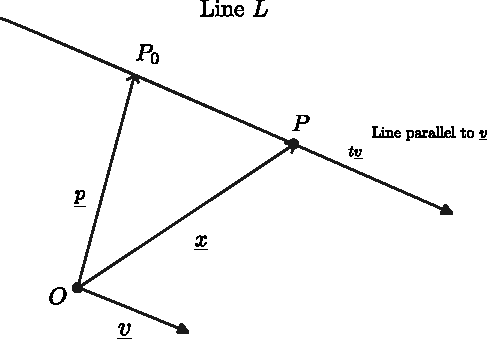
\includegraphics[scale=1.0]{vector-lines.pdf}
	\caption{Vector Line}
	\label{fig:figure-vector-lines}
\end{figure}

\subsection{Parametric Equation of a Line}
\begin{note}
	Every point $\underline{x}$ can be written as
	$$\underline{x} = x\hat{i} + y\hat{j} + z\hat{k}$$
	Therefore we can form a parametric equation of a line
\end{note}

\begin{definition}[Parametric Equation of a Line]
	\begin{equation}
		\label{eq: parametric-vector-lines}
		\begin{cases}
			x = x_0 + tv_1 \\
			y= y_0 + tv_2  \\
			z = z_0 + tv_3
		\end{cases}
		\ \ \ \ \ \text{for } t \in \mathbb{R}
	\end{equation}

\end{definition}

\subsection{Vector Equation of Line going through 2 points}
\begin{definition}
	Let $P$ and $Q$ be two points on the line and let their position vectors be $\underline{p}$ and $\underline{q}$ repectively. Then the
		{\bf direction vector} is:
	$$\vec{PQ} = \underline{q} - \underline{p}$$
	and the vector equation line is
	\begin{equation}
		\label{eq vector-lines-2p}
		\underline{x} = + t(\underline{q} - \underline{p}) \ \ \ \ \text{for } t \in \mathbb{R}
	\end{equation}
\end{definition}
The following diagram depicts this:

\begin{figure}[H]
	\centering
	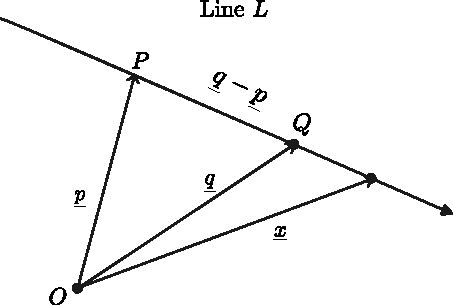
\includegraphics[scale=1.0]{vector-lines-2p.pdf}
	\caption{Vector Line}
	\label{fig:figure-vector-lines-2p}
\end{figure}
